\chapter{Introduction}\label{ch:introduction}

\vspace*{-50pt}

\begin{figure}[ht]
        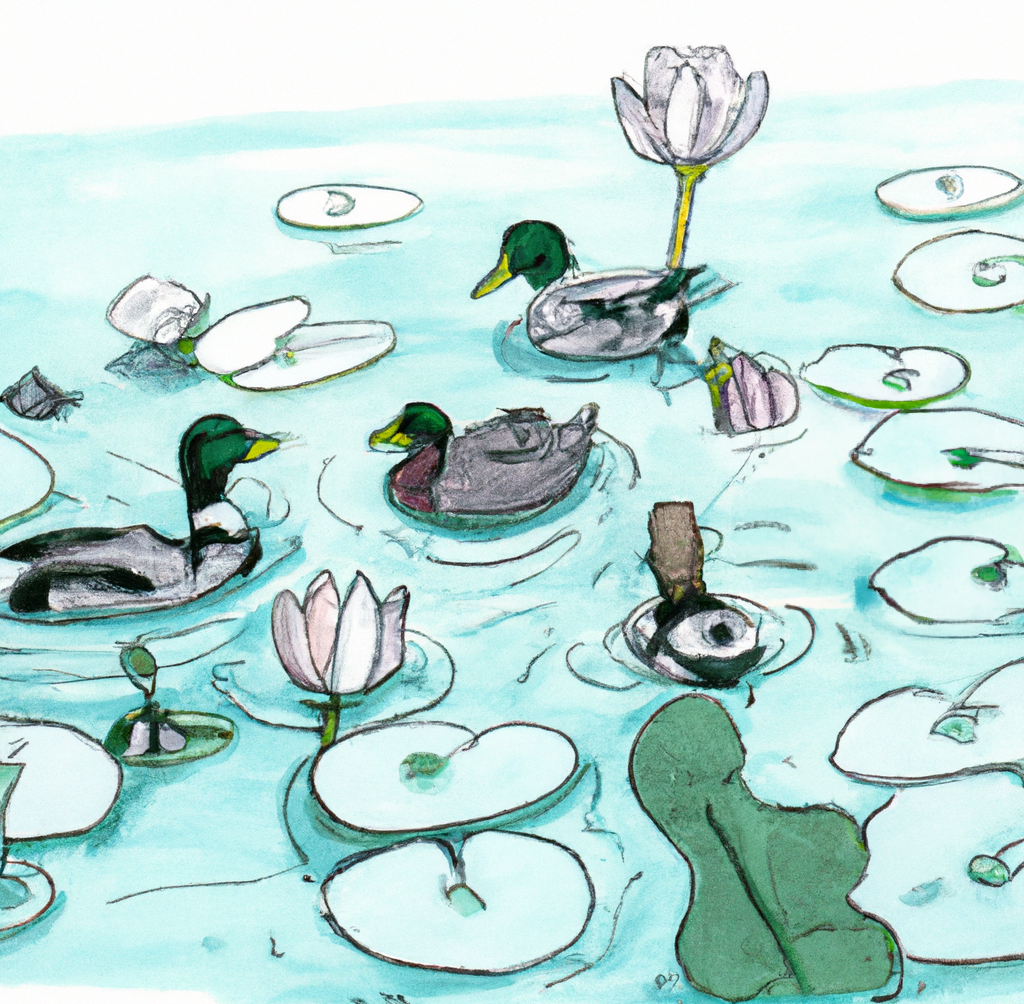
\includegraphics[width=0.35\textwidth, right]{img/dalle-ducks.png}
        \captionsetup{textformat=empty,labelformat=blank}
        \caption{Generated with Dall-E. \url{https://labs.openai.com/}. ``A duck dominating sitting on a searose''}
\end{figure}

\epigraph{\itshape Todo select another quote}{Lewis Caroll, \textit{XXXX}}

\begin{wrapfigure}{R}{0.35\textwidth}
\end{wrapfigure}

Parametrized Complexity emerging branch. Books about that

Semitotal domination was introduced by 
% TODO: Idea for a nice introduction 

Quack! Quack! Idea:  Lake with stones, and a family of ducks of fixed size want to occupy the lake so that no other clan tries to take it over.
Rules: 
* A duck can quack freeing up neighboring stones.
* Ducks don't like to be alone and want to quack together. So for every duck their must be another duck that is not further than two stones away.
Q: Can our ducklings occupy the whole lake while not feeling lonely?


TODO A demo instance next to each other 

\section{Content of the thesis}

In this thesis, we continue the systematic analysis of the \sdom problem by focusing on the parametrized complexity of the problem. 

Although the problem already had a lot of attention regarding classical complexity (CITE), only a few results are currently known for the parametrized variant. 

As far as we have seen, even the w-hardness of the general case has not been explicitly been proven in the literature. 

In this thesis, we continue the journey toward a systematic analysis by stating some hardness results for specific graph classes for the problem.

\paragraph{Our contributions}
% TODO Better: 

Our main contributions consist of first showing the $w[2]$-hardness of \sdom for XXXX graphs.

\noindent As the \dom problem and the \tdom problem both admit a linear kernel for planar graphs, it is interesting to analyse wether this results also holds for the \sdom problem which lays in between these two. 
%TODO by relxing the witness of these two provlemsproblems.

Having these kernels also for other variants like \eddom, \efdom, \cdom, \rbdom lent us great confidence that the result will also work for \sdom on planar graphs.

%% TODO Find more  .

Following the approach from ... which already relies on the technique given in, we give some simple data reduction rules for \sdom on planar graphs leading to a linear kernel. More precisely, we are going to proof the following central theorem of this thesis:

With some modifications, we were able to transfer the approach given by Garnero and Sau in \cite{Garnero2018} to the \sdom problem.

\begin{restatable}[]{theorem}{centraltheo}\label{thm:central}
    The \sdom problem parametrized by solution size admits a linear kernel on planar graphs. There exists a polynomial-time algorithms that given a planar graph $(G, k)$, either correctly reports that $(G, k)$ is a NO-instance or returns an equivalent instance $(G', k)$ such that $\abs{V(G')} \leq \kernelsize \cdot k$.
\end{restatable}

\dom problem and \tdom problem, both already 

